% Provenance (never printed): old terminale S material on the Earth's internal
% heat (geothermal gradient and heat flow, radioactive heat production,
% conduction and convection, mantle convection, geothermal energy). Owner
% (Sync 0/1): heat flow, radiogenic heat production, secular cooling, thermal
% and mantle convection (recall the convection cell of Book 1 g8 first),
% geothermal energy. Geotherm and geothermal gradient are g11.03's; radioactivity,
% half-life, decay law and thermal conductivity are physics' (thermal
% conductivity used as "the rock's thermal conductivity k", never defined);
% hotspot track and plume g11.04's. Figures: figdata/grade-12/internal_heat.py.
\chapter{地球的内部热量}\label{ch:g12:internal-heat}

1987 年至 1995 年间，在巴伐利亚的温迪施埃申巴赫村附近，
地质学家在\omterm{def:g12:continental-crust:continental-crust}{大陆地壳}中钻了一个深 \qty{9101}{m} 的钻孔。钻孔
底部岩石温度约为 \qty{265}{\celsius}，已经太热，无法
继续向下钻探。
% ledger: gfz:ktb, gfz:ktb30

从地表约 \qty{10}{\celsius} 升至
\qty{9.1}{km} 深处的 \qty{265}{\celsius}，即每千米约升温 \qty{28}{\celsius}，这是一个典型值。
地球各处都是越往深处越热，因此热量
持续从地球内部向外流出。本章测量这种\omterm{def:g12:internal-heat:heat-flow}{热流}，探讨热量
的来源，并说明热量如何运动。
% values: ktb_gradient 28.0 (internal_heat.py, surface temperature taken as 10 degC); ledger: gfz:ktb (gradient about 28 K/km)

\begin{recall}
\omterm{def:g11:lithosphere-asthenosphere:geotherm}{地温线}是某地下方温度随深度变化的曲线，
\omterm{def:g11:lithosphere-asthenosphere:geotherm}{地温梯度}是每千米温度的升高量；钻孔
在近地表处，钻孔测得的值为每千米 \qty{25}{\celsius} 至 \qty{30}{\celsius}
（见\cref{ch:g11:lithosphere-asthenosphere}）。某些原子具有放射性，它们
随机衰变，剩余原子数每经过一个半衰期减半，每次
衰变都会释放能量，这些能量最终转化为热量（参见物理教材）。一个
对流环流是一个流体环路，流体从下方受热，上升、扩散、
冷却后下沉（第 1 册，八年级）。在热点处，板块
正经过一个热地幔柱上方（见\cref{ch:g11:plate-motions}）。
\end{recall}
% ledger: usgs:gradient-29 (Book 1 row)

\section{梯度与热流}

\begin{definition}[热流]\label{def:g12:internal-heat:heat-flow}
某地的\emph{热流}\index{热流}（或热\omterm{def:g10:drainage-basins:discharge}{流量}）是
从地球内部经该处地表每平方米流出的功率。
通常以毫瓦每平方米计量，
即 \unit{mW/m^2}。
\end{definition}
% ledger: b2dd10:continents

热量从热处流向冷处，温度梯度越陡，
\omterm{def:g12:internal-heat:heat-flow}{热流}越快。\omterm{def:g12:internal-heat:heat-flow}{热流}的大小还取决于岩石：每种岩石都有一个
热导率 $k$（单位为瓦每米每开尔文），
由物理教材给出定义。

\begin{proposition}[热流与梯度]\label{prop:g12:internal-heat:fourier}
设热导率为 $k$ 的岩石中，温度随深度
以梯度 $G$（单位为开尔文每米）升高，则向上流向
地表的\omterm{def:g12:internal-heat:heat-flow}{热流}为
\[
  q = k\,G .
\]
\end{proposition}

这一传导定律由傅里叶提出，在本阶段不加证明地承认；
物理教材会证明其一般形式。

\begin{method}[由钻孔测定热流]\label{met:g12:internal-heat:borehole}
\begin{enumerate}
  \item 测量钻孔中若干深度处的温度，待钻孔
        温度恢复到与岩石温度一致之后进行。
  \item 以深度为横轴、温度为纵轴作图，取斜率即为梯度 $G$，
        并换算为开尔文每米。
  \item 在实验室中，用岩芯测量岩石的
        热导率 $k$。
  \item 相乘：$q = kG$，单位为 \unit{W/m^2}，再换算为 \unit{mW/m^2}。
\end{enumerate}
\end{method}

\begin{example}[花岗岩中的钻孔]\label{ex:g12:internal-heat:borehole}
某花岗岩中的钻孔，热导率为 \qty{2.72}{W/(m.K)}，测得
梯度为每千米 \qty{29}{\celsius}，即 \qty{0.029}{K/m}。
于是 $q = 2.72 \times 0.029 \approx \qty{0.079}{W/m^2}$，约
合 \qty{79}{mW/m^2}。
\end{example}
% ledger: roy:conductivity (granitic layer 6.5 mcal/(cm s degC) = 2.72 W/m/K), usgs:gradient-29 (Book 1 row)
% values: borehole_q_mW 78.9 (internal_heat.py)

已有超过 38\,000 次此类测量被汇总为一幅
全球\omterm{def:g12:internal-heat:heat-flow}{热流}图。大陆平均\omterm{def:g12:internal-heat:heat-flow}{热流}为 \qty{70.9}{mW/m^2}，洋底
为 \qty{105.4}{mW/m^2}；全部地表的平均值为 \qty{91.6}{mW/m^2}。
乘以地球表面积 \qty{5.101e14}{m^2}，总量为
\[
  0.0916 \times \num{5.101e14} \approx \qty{4.67e13}{W} = \qty{46.7}{TW},
\]
约 47 太瓦，上下浮动约 2 太瓦。
% ledger: b2dd10:continents, b2dd10:half-space (47 +- 2 TW, 38,347 measurements)

洋底在最年轻的地方失热最多。新生\omterm{def:g11:lithosphere-asthenosphere:lithosphere}{岩石圈}离开洋脊时温度很高，
随远离洋脊而冷却；其\omterm{def:g12:internal-heat:heat-flow}{热流}
与年龄的平方根成反比减小。

\begin{omfigure}
\begin{tikzpicture}
\begin{axis}[omrecord, width=0.72\linewidth, height=5.6cm, xmin=0, xmax=180, ymin=0, ymax=400,
  xlabel={洋底年龄（百万年）}, ylabel={热流（\unit{mW/m^2}）},
  xtick={0,30,...,180}, ytick={0,100,...,400}]
% computed in figdata/grade-12/internal_heat.py; ledger: b2dd10:half-space, b2dd10:continents
\addplot[omDef, line width=1.1pt, restrict x to domain=0:66.5] table[x=t_Myr, y=q] {figdata/out/grade-12-internal_heat-halfspace.dat};
\addplot[omDef, line width=1.1pt, densely dotted, restrict x to domain=66.5:180] table[x=t_Myr, y=q] {figdata/out/grade-12-internal_heat-halfspace.dat};
\addplot[omProp, line width=0.9pt, dashed, domain=0:180] {70.9};
\coordinate (lawlab) at (axis cs:14,250);
\coordinate (contlab) at (axis cs:100,80);
\end{axis}
\node[font=\scriptsize, text=omDef, anchor=west] at (lawlab) {$q = 490/\sqrt{t}$};
\node[font=\scriptsize, text=omProp, anchor=south west] at (contlab) {大陆平均值，\qty{70.9}{mW/m^2}};
\end{tikzpicture}

{\small 海底\omterm{def:g12:internal-heat:heat-flow}{热流}随其年龄的变化，依据
\omterm{def:g11:lithosphere-asthenosphere:lithosphere}{岩石圈}冷却所作的计算（$t$ 以百万年计）；超过 66.5
百万年（虚线）后，该规律的拟合效果已知较差。来源：Davies
and Davies（2010）。}
\end{omfigure}
% values: q_1Myr 490, q_10Myr 155, q_66.5Myr 60.1, age_where_q_equals_cont_Myr 47.8 (internal_heat.py)

\section{热量的来源}

热量有两个来源。第一个来源是放射性。

\begin{definition}[放射性生热]\label{def:g12:internal-heat:heat-production}
称岩石的\emph{放射性生热}\index{放射性生热}
为其内部因放射性原子衰变而释放的热量，
单位体积、单位时间内，以微瓦每立方米计
（\unit{\micro W/m^3}）。几乎全部来自四种同位素：铀-238、
铀-235、钍-232 和钾-40。
\end{definition}
% ledger: dye12:isotopes, earle:heat-sources, kamland11:geonu

这些元素集中于\omterm{def:g12:continental-crust:continental-crust}{大陆地壳}的岩石中。
依据 2188 个分析结果，花岗岩\omterm{def:g12:internal-heat:heat-production}{放射性生热}的中位数为
\qty{2.43}{\micro W/m^3}，玄武岩为 \qty{0.21}{\micro W/m^3}，而地幔
超\omterm{def:g11:igneous-rocks:felsic-mafic}{镁铁质}岩仅为 \qty{0.11}{\micro W/m^3}，约
比花岗岩低二十倍。厚 \qty{10}{km} 的花岗岩层
每平方米产生的功率约为 $2.43 \times 10^{-6} \times \num{10000} \approx \qty{0.024}{W}$，
即 \qty{24}{mW/m^2}：约占大陆\omterm{def:g12:internal-heat:heat-flow}{热流}的三分之一。
% ledger: b2vila:heat-production, b2dd10:continents
% values: granite_10km_mW 24.3, granite_over_ultramafic 21.9 (internal_heat.py)

放射性在整个地球中产生多少热量？KamLAND 是
位于日本地下、装有 1000 吨液体的探测器，用来捕获
地中微子，即铀和钍在地球内部衰变时释放的反中微子：
它于 2005 年首次探测到地中微子，在 2135 天的记录中，
841 个候选事件中约有 106 个。由此计数，
结合意大利探测器的数据，铀-238 和钍-232 合计
释放约 20 太瓦。钾-40 不被探测器捕获；据已知，
它约增加 \qty{4}{TW}，铀-235 按铀-238 换算，约
\qty{0.4}{TW}。因此，放射性提供约 \qty{24}{TW}，
约占地球散失热量 \qty{47}{TW} 的一半。
% ledger: kamland11:geonu, dye12:isotopes, b2dd10:continents
% values: now_K40_TW 4.0, now_U235_TW 0.42, radiogenic_TW 24.4, share_radiogenic 0.523 (internal_heat.py)

\begin{definition}[长期冷却]\label{def:g12:internal-heat:secular-cooling}
称地球的\emph{长期冷却}\index{长期冷却}为
地球自形成以来储存于内部的原始热量的缓慢散失，即
\omterm{def:g12:internal-heat:heat-flow}{热流}中未被\omterm{def:g12:internal-heat:heat-production}{放射性生热}所补偿的部分，
由此使地幔和地核随时代推移而逐渐变冷。
\end{definition}
% ledger: kamland11:geonu, earle:heat-sources

\begin{omfigure}
\begin{tikzpicture}
\begin{axis}[omrecord, xbar stacked, bar width=14pt, width=0.66\linewidth, height=3.2cm, scale only axis,
  xmin=0, xmax=50, ymin=0.4, ymax=2.6, ytick={1,2}, yticklabels={{来源}, {损失}},
  xlabel={功率（\unit{TW}）}, ymajorgrids=false, legend columns=2, legend cell align=left,
  legend style={font=\scriptsize, at={(0.5,-0.42)}, anchor=north, /tikz/every even column/.append style={column sep=6pt}}]
% computed in figdata/grade-12/internal_heat.py; ledger: kamland11:geonu, dye12:isotopes, b2dd10:continents
\addplot[fill=omThm!55, draw=omThm] table[x=uth, y=bar] {figdata/out/grade-12-internal_heat-budget.dat};
\addplot[fill=omThm!25, draw=omThm] table[x=kuf, y=bar] {figdata/out/grade-12-internal_heat-budget.dat};
\addplot[fill=omDef!35, draw=omDef] table[x=secular, y=bar] {figdata/out/grade-12-internal_heat-budget.dat};
\addplot[fill=black!25, draw=black!60] table[x=surface, y=bar] {figdata/out/grade-12-internal_heat-budget.dat};
\legend{{铀-238 和钍-232（地中微子）}, {钾-40 和铀-235}, {长期冷却（其余部分）}, {地表热流}}
\end{axis}
\end{tikzpicture}

{\small 今日地球的热量收支：自地表散失的热量（上方条）
以及为其补给的热量（下方条）。来源：KamLAND（2011）；Davies 和 Davies
（2010）；Dye（2012）。}
\end{omfigure}
% values: radiogenic_TW 24.4, secular_TW 22.3 (internal_heat.py)

过去的放射性更强。每种同位素都会衰变，因此
很久以前它的量更多：回溯一个半衰期，量为两倍，
热量也为两倍。回溯 $t$ 年，半衰期为
$T$ 的同位素的热量乘以 $2^{t/T}$。

\begin{proposition}[过去的放射性生热]\label{prop:g12:internal-heat:past}
若半衰期为 $T$ 的同位素今日释放的功率为 $H_0$，则其
\[
  H(t) = H_0 \, 2^{t/T} = H_0\, e^{\lambda t}, \qquad \lambda = \frac{\ln 2}{T},
\]
即 $t$ 年前的释放功率。
\end{proposition}

\begin{proof}
功率与尚存的原子数 $N$ 成正比，因为每个原子
每秒衰变的概率相同。由衰变律，$N$ 每经过
一个半衰期减半：$N_{\text{现在}} = N(t)\,2^{-t/T}$，于是 $N(t) =
N_{\text{现在}}\,2^{t/T}$，功率随之得出。最后，$2^{t/T} =
e^{(t/T)\ln 2} = e^{\lambda t}$。
\end{proof}

\begin{omfigure}
\begin{tikzpicture}
\begin{axis}[omrecord, width=0.72\linewidth, height=6cm, xmin=0, xmax=4.5, ymin=0, ymax=120,
  x dir=reverse, xlabel={距今时间（十亿年）}, ylabel={放射性生热（\unit{TW}）},
  xtick={0,0.5,...,4.5}, ytick={0,20,...,120}, x tick label style={/pgf/number format/.cd, fixed, precision=1},
  legend pos=north east, legend style={font=\scriptsize}, legend cell align=left]
% computed in figdata/grade-12/internal_heat.py; ledger: kamland11:geonu, dye12:isotopes, nndc:halflives
\addplot[black, line width=1.2pt] table[x=t_Ga, y=total] {figdata/out/grade-12-internal_heat-past.dat};
\addplot[omThm, line width=0.9pt] table[x=t_Ga, y=U235] {figdata/out/grade-12-internal_heat-past.dat};
\addplot[omProp, line width=0.9pt, densely dashed] table[x=t_Ga, y=K40] {figdata/out/grade-12-internal_heat-past.dat};
\addplot[omDef, line width=0.9pt] table[x=t_Ga, y=U238] {figdata/out/grade-12-internal_heat-past.dat};
\addplot[omMeth, line width=0.9pt, densely dotted] table[x=t_Ga, y=Th232] {figdata/out/grade-12-internal_heat-past.dat};
\legend{总量, 铀-235, 钾-40, 铀-238, 钍-232}
\end{axis}
\end{tikzpicture}

{\small 四种放射性同位素回溯至地球形成时所释放的热量，
依据今日数值，由衰变律推算。半衰期：
钍-232 为 14.0 十亿年；铀-238 为 4.468；钾-40 为 1.248；
铀-235 为 0.704。}
\end{omfigure}
% values: total_4.5Ga_TW 115.9, ratio_total_4.5Ga 4.75, ratio_U235_4.5Ga 84.0, ratio_K40_4.5Ga 12.2, share_U235_K40_4.5Ga 0.72 (internal_heat.py)

四十五亿年前，放射性释放的热量约为
\qty{116}{TW}，几乎是今日数值的五倍，其中大部分来自
铀-235 和钾-40 这两种短寿命同位素，它们此后
几乎已经耗尽。年轻地球的内部比今天热得多。
% ledger: earle:heat-sources (radiogenic heat now roughly 25 % of what it was)

\section{传导与对流}

热量只能借传导穿过固体，即从一个原子传到另一个原子，而在岩石中
这一过程极其缓慢。热量借传导穿过距离 $L$ 所需的时间
约为 $L^2/\kappa$，其中 $\kappa$ 为岩石的热扩散率，
约为 \qty{1e-6}{m^2/s}。对于地幔的
\qty{2891}{km}，
\[
  \frac{(\num{2.891e6})^2}{\num{1e-6}} \approx \qty{8.4e18}{s} \approx
  \num{2.6e11} \text{ 年},
\]
约 2600 亿年，几乎是地球年龄的六十倍。若地幔
只靠传导传递热量，其深处的热量仍几乎全部保留。
% ledger: england:kelvin (Book 3 row: kappa 1e-6 m2/s), data:prem (CMB at 2891 km)
% values: conduction_time_Gyr 264.9 (internal_heat.py)

地幔是固体，但在数百万年的时间尺度上，它会极其缓慢地蠕动，
像一种非常黏稠的流体：\omterm{def:g11:lithosphere-asthenosphere:lithosphere}{软流圈}发生流动（见\cref{ch:g11:lithosphere-asthenosphere}）。
因此，地幔散失热量的方式与暖气片上方的空气相同，靠携带热量来完成。

\begin{definition}[热对流；地幔对流]\label{def:g12:internal-heat:convection}
\emph{热对流}\index{热对流}是借物质自身运动而输运热量的过程：
较热、较轻的物质上升，
较冷、较重的物质下沉，形成对流环流。
\emph{地幔对流}\index{地幔对流}是地球固态地幔中的热
对流，地幔以每年几厘米的速度缓慢蠕动，
把地球内部的热量输运到表面。
\end{definition}
% ledger: earle:heat-sources (solid mantle flows at centimetres a year)

板块是这一对流的上部。在洋脊处，热的地幔物质
上升并加入板块；\omterm{def:g11:lithosphere-asthenosphere:lithosphere}{岩石圈}在远离洋脊的过程中冷却，
变密，在\omterm{def:g11:subduction-zones:subduction}{俯冲带}因自身重量而下沉：\omterm{def:g11:subduction-zones:slab}{板片}
是流动中冷而下沉的部分，地震成像显示它们
深入地幔之中。据信，热点之下的热柱
自地幔深处升起，可能起源于地核正上方。
% ledger: dye12:bse, earle:plume

\begin{omfigure}
\begin{tikzpicture}[x=1cm, y=1cm, font=\scriptsize]
  % mantle annulus sector
  \fill[omLithPeridotite!40] (0,0) ++(20:6.4) arc (20:160:6.4) -- ++(160:-3.2) arc (160:20:3.2) -- cycle;
  \fill[black!45] (0,0) ++(20:3.2) arc (20:160:3.2) -- (0,0) -- cycle;
  \node[white] at (0,1.6) {地核};
  % lithosphere
  \fill[black!15, draw=black!50] (0,0) ++(20:6.4) arc (20:160:6.4) -- ++(160:-0.3) arc (160:20:6.1) -- cycle;
  % ridge (top) and two trenches
  \draw[omThm, line width=1pt, -{Stealth}] (0,5.9) -- (0,6.35);
  \node[anchor=south] at (0,6.45) {洋脊};
  \foreach \a/\lab in {48/海沟, 132/海沟} {
    \node[anchor=south] at (\a:6.5) {\lab};
  }
  % slabs (cold, blue) sinking from the trenches
  \draw[omDef, line width=3pt] (48:6.2) .. controls (52:5.2) and (60:4.4) .. (62:3.4);
  \draw[omDef, line width=3pt] (132:6.2) .. controls (128:5.2) and (120:4.4) .. (118:3.4);
  % plume (hot, red) rising
  \draw[omThm, line width=2.4pt] (155:3.25) .. controls (154:4.2) and (152:5.2) .. (151:6.05);
  \fill[omThm] (151:6.0) circle (0.18);
  \node[anchor=west, text=omThm] at (145:4.0) {热柱？};
  % convection arrows
  \draw[-{Stealth}, black!65, line width=0.8pt] (80:5.7) arc (80:58:5.7);
  \draw[-{Stealth}, black!65, line width=0.8pt] (100:5.7) arc (100:122:5.7);
  \draw[-{Stealth}, black!65, line width=0.8pt] (68:3.7) .. controls (80:3.6) and (88:4.5) .. (90:5.4);
  \draw[-{Stealth}, black!65, line width=0.8pt] (112:3.7) .. controls (100:3.6) and (92:4.5) .. (90:5.4);
  \node[omDef, anchor=north west, align=left] at (52:4.55) {冷板片 \\下沉};
  \node[anchor=north, white] at (90:2.95) {核幔边界};
  \node[anchor=south east] at (150:6.45) {板块};
\end{tikzpicture}

{\small \omterm{def:g12:internal-heat:convection}{地幔对流}（示意图，未按比例绘制）。板块是其冷的
上边界：热的地幔物质在洋脊下方上升，板块在远离洋脊时冷却，
并以\omterm{def:g11:subduction-zones:slab}{板片}的形式在海沟处下沉回地幔，其中一些深入下地幔。
热柱可能自地幔深处在热点之下升起。}
\end{omfigure}
% ledger: dye12:bse, earle:plume

因此，热量大部分借对流离开地幔，只有最后
几十千米，穿过刚性的\omterm{def:g11:lithosphere-asthenosphere:lithosphere}{岩石圈}时，才以传导方式输运——
即钻井所测量的那种传导。
% ledger: dye12:bse (convection the main transport of interior heat), earle:heat-sources

\section{地热能}

\begin{definition}[地热能]\label{def:g12:internal-heat:geothermal}
\emph{地热能}\index{地热能}是人类利用的地球内部热量：
来自热岩的热水或蒸汽，经水井被抽取上来，
用于供暖或发电。
\end{definition}
% ledger: eia:geo-use, eia:geo-plants

从地球向外流出的热量，到达地表时极其微弱，
每平方米约 \qty{0.1}{W}，远不足以直接利用。它
只有在较浅的深度上集中时，才变得可以利用。在火山、
裂谷和热点附近，以及沿板块边界，热岩靠近
地表，在透水岩石中循环的水又以热水的形式回流。发电
厂需要温度很高的热水或蒸汽，约为 150 至
\qty{370}{\celsius}；某些地热田产出干蒸汽，
直接驱动涡轮机。人类首次利用地球热量发电是在 1904 年，地点在
托斯卡纳的拉德雷洛，它点亮了五个灯泡。在其他地方，
近地表的热水被输送至建筑物内用于供暖。
% ledger: b2dd10:continents, eia:geo-where, eia:geo-plants (300 to 700 degF), enel:larderello, eia:geo-use

\begin{omfigure}
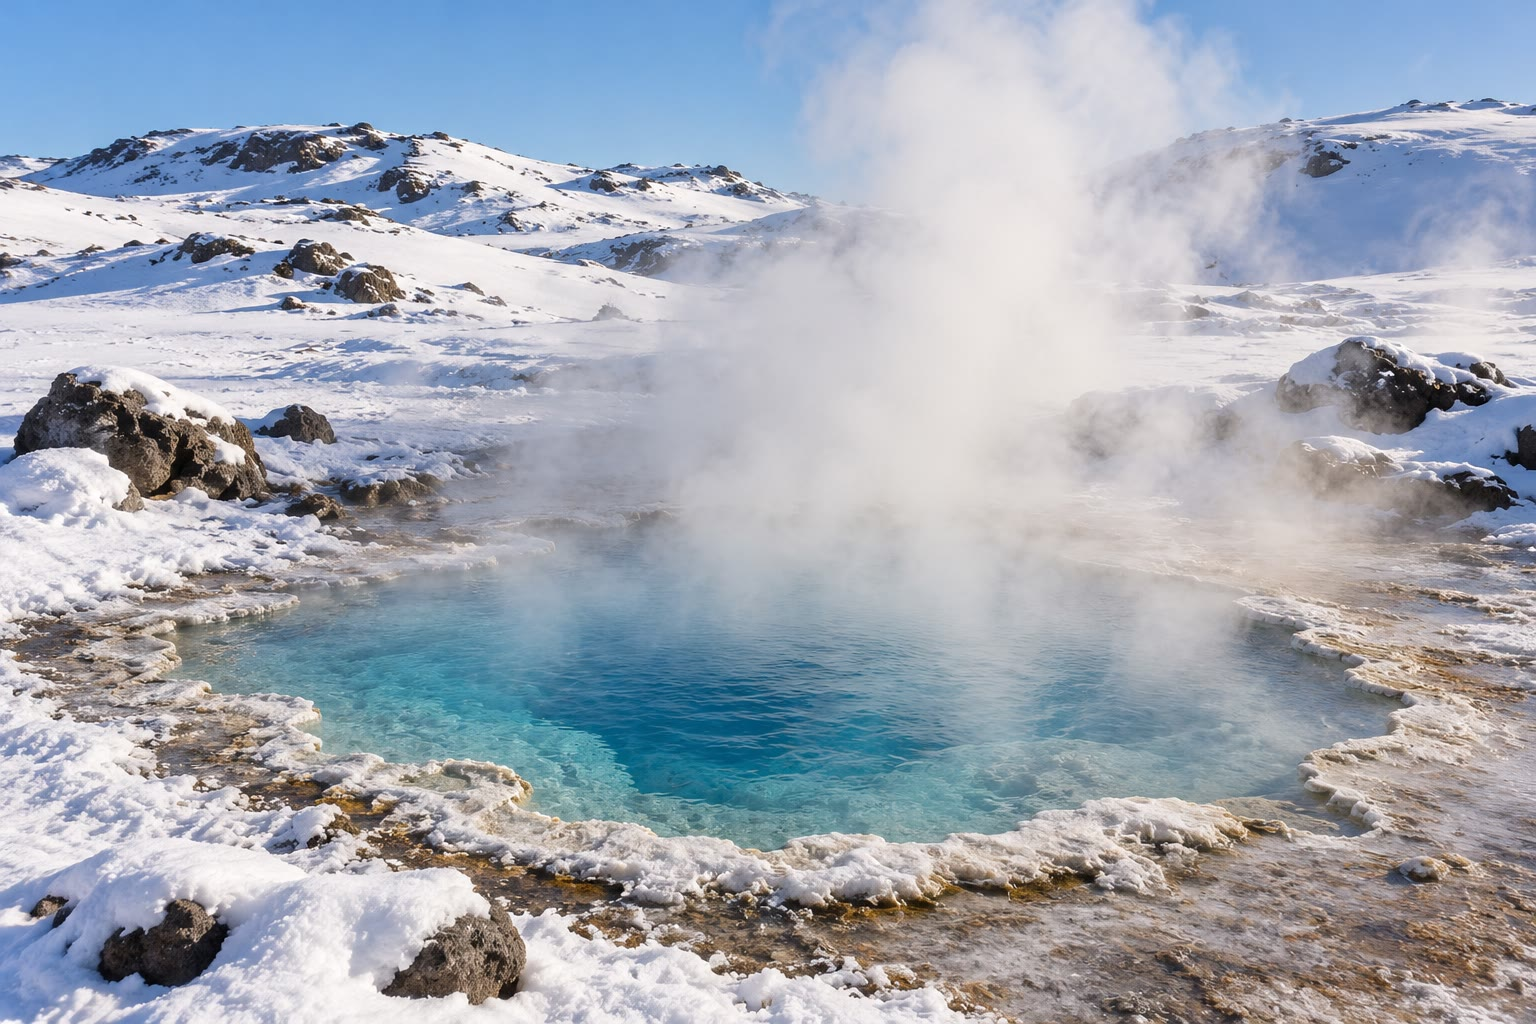
\includegraphics[width=0.6\linewidth]{images/book2/ai/g12-hot-spring-snow.jpg}

{\small 雪景中冒着蒸汽的温泉：地下深处被加热的水
重新回到地表。AI 生成的插图。}
\end{omfigure}

\begin{omfigure}
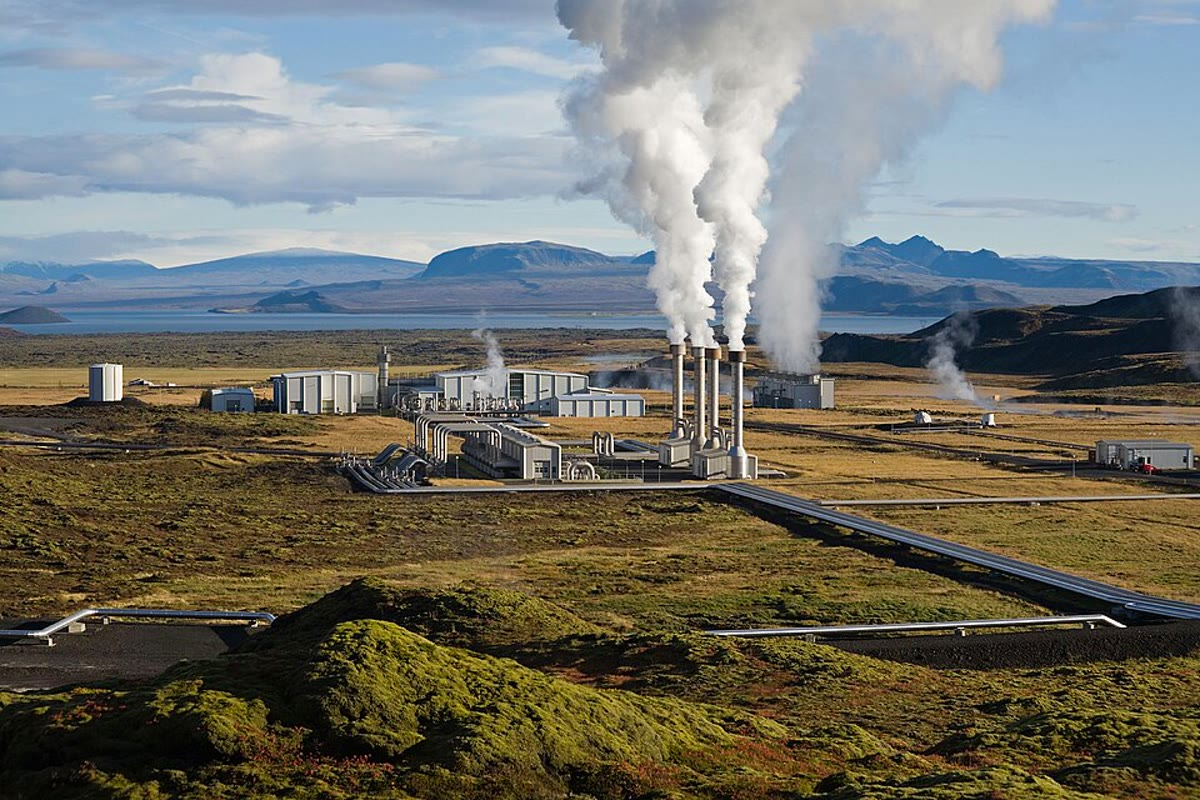
\includegraphics[width=0.66\linewidth]{images/book2/g12-nesjavellir-geothermal.jpg}

{\small 位于冰岛火山区亨吉尔的内斯耶利尔地热电站：
最大电功率可达 \qty{120}{MW}，最大热功率可达
\qty{300}{MW}，热量由热水输送。照片：Gretar
Ívarsson，公有领域。}
\end{omfigure}
% ledger: photo:g12-nesjavellir, on:nesjavellir

地热田在人类寿命的尺度上并非取之不尽。
加利福尼亚的间歇泉地热田，抽汽井过多，
抽取蒸汽的速度超过了缓慢的\omterm{def:g12:internal-heat:heat-flow}{热流}与降雨的补给：
蒸汽压强降至峰值的一半以下，发电厂容量
损失超过 \qty{40}{\percent}。目前向地热田回注水，
以减缓衰减。
% ledger: cpuc:geysers

\section{练习}

\begin{exercise}[$\star$]\label{exo:g12:internal-heat:1}
写出下列各项对应的术语：(a) 通过每平方米地表从内部
向外输出的功率；(b) 岩石单位体积内放射性原子衰变释放的热量；
(c) 地球形成以来所储存热量的损失；
(d) 物质自身运动输送热量的方式；
(e) 人类利用的地球内部热能。
\end{exercise}

\begin{exercise}[$\star$]\label{exo:g12:internal-heat:2}
换算下列各量：(1) 将 \qty{91.6}{mW/m^2} 换算为 \unit{W/m^2}；(2) 将 \qty{46.7}{TW} 换算为
瓦特；(3) 将每千米 \qty{29}{\celsius} 换算为每米开尔文。
\end{exercise}

\begin{exercise}[$\star$]\label{exo:g12:internal-heat:3}
写出产生几乎全部\omterm{def:g12:internal-heat:heat-production}{放射性生热}的四种同位素，并说明
KamLAND 探测器能够探测到其中哪两种。
\end{exercise}

\begin{exercise}[$\star$]\label{exo:g12:internal-heat:4}
利用 $q = 490/\sqrt{t}$，计算年龄为
1、4、25 和 49 百万年的洋底所通过的\omterm{def:g12:internal-heat:heat-flow}{热流}。
\end{exercise}

\begin{exercise}[$\star$]\label{exo:g12:internal-heat:5}
为什么\omterm{def:g12:internal-heat:heat-flow}{热流}要在钻孔中测量，而不在地表直接测量？
为什么钻孔完成后必须等待一段时间才能测量？
\end{exercise}

\begin{exercise}[$\star\star$]\label{exo:g12:internal-heat:6}
在 KTB 钻孔中，岩石温度约为
\qty{265}{\celsius}，深度为 \qty{9.1}{km}。(1) 取地表温度为 \qty{10}{\celsius}，计算平均
梯度；(2) 若热导率为 \qty{2.72}{W/(m.K)}，求由此得到的\omterm{def:g12:internal-heat:heat-flow}{热流}；
(3) 与大陆平均值相比较。
\end{exercise}

\begin{exercise}[$\star\star$]\label{exo:g12:internal-heat:7}
大陆覆盖面积 \qty{2.073e14}{m^2}，平均\omterm{def:g12:internal-heat:heat-flow}{热流}为
\qty{70.9}{mW/m^2}；海洋面积 \qty{3.028e14}{m^2}，平均\omterm{def:g12:internal-heat:heat-flow}{热流}为
\qty{105.4}{mW/m^2}。计算大陆与海洋各自散失的功率及总功率，
以及经洋底散失的份额。
\end{exercise}

\begin{exercise}[$\star\star$]\label{exo:g12:internal-heat:8}
一层厚 \qty{8}{km} 的\omterm{def:g12:subduction-magmatism:granodiorite}{花岗闪长岩}，其生热率为
\qty{1.88}{\micro W/m^3}。(1) 该层在地表产生的\omterm{def:g12:internal-heat:heat-flow}{热流}是多少？
(2) 它占 \qty{70.9}{mW/m^2} 的份额是多少？
\end{exercise}

\begin{exercise}[$\star\star$]\label{exo:g12:internal-heat:9}
洋底在何种年龄时失去的热量与平均大陆
\qty{70.9}{mW/m^2} 相同，依据 $q = 490/\sqrt{t}$？
\end{exercise}

\begin{exercise}[$\star\star$]\label{exo:g12:internal-heat:10}
铀-235 在 14 亿年前释放的热量比今天多多少？
钾-40 在 25 亿年前比今天多释放的热量又是多少？
\end{exercise}

\begin{exercise}[$\star\star$]\label{exo:g12:internal-heat:11}
利用 $t \approx L^2/\kappa$，其中 $\kappa = \qty{1e-6}{m^2/s}$，求热量
通过传导穿过下列各层所需的时间：(1) 厚 \qty{10}{m} 的熔岩流；
(2) 厚 \qty{100}{km} 的\omterm{def:g11:lithosphere-asthenosphere:lithosphere}{岩石圈}；(3) 地幔。请用合适的单位
表示每个结果。
\end{exercise}

\begin{exercise}[$\star\star\star$]\label{exo:g12:internal-heat:12}
今天钍-232 释放约 \qty{10.4}{TW}，铀-238 释放 \qty{9.6}{TW}，
钾-40 释放 \qty{4.0}{TW}，铀-235 释放 \qty{0.42}{TW}。利用图中的
半衰期，计算 30 亿年前每种同位素释放的热量，
求其总和，以及两种短寿命同位素
所占的份额。
\end{exercise}

\begin{exercise}[$\star\star\star$]\label{exo:g12:internal-heat:13}
内斯耶利尔电站最多可输出 \qty{300}{MW} 的热量，
由每秒约 \qty{1640}{L} 的热水携带。已知比热容为 \qty{4180}{J/(kg.K)}，
每升水的质量为 \qty{1}{kg}，这些水升温了多少度？
求平均大陆区域损失
\qty{300}{MW} 热量时所对应的面积。
\end{exercise}

\begin{exercise}[$\star\star\star$]\label{exo:g12:internal-heat:14}
假设一个板块从洋脊运动到海沟需要 1 亿年，一次贯穿整个地幔的
对流环流约需 2 亿年。(1) 将这些时间与热量经传导穿越地幔所需的
2600 亿年相比较。
(2) 为何对流输送热量的速度远快于此，
即使地幔每年仅移动几厘米？
\end{exercise}

\begin{exercise}[$\star\star\star$]\label{exo:g12:internal-heat:15}
假设地核向地幔散失约 \qty{10}{TW} 的热量，热量穿过
\omterm{def:g11:seismic-structure:core}{核幔边界}，该边界位于地下 \qty{2891}{km} 处。(1) 这相当于
\omterm{def:g12:internal-heat:secular-cooling}{长期冷却} \qty{22.3}{TW} 的多大份额？其余部分
来自何处？(2) 求穿过\omterm{def:g11:seismic-structure:core}{核幔边界}的
平均\omterm{def:g12:internal-heat:heat-flow}{热流}，并与地表的平均\omterm{def:g12:internal-heat:heat-flow}{热流}
相比较，其值为 \qty{91.6}{mW/m^2}。(3) 为何炽热的地核
能够加热地幔底部，尽管地幔是固体？
\end{exercise}

\begin{problem}[{周末问题——地球的热量收支}]
\label{pb:g12:internal-heat:1}
% ledger: b2dd10:continents, b2dd10:half-space, kamland11:geonu, dye12:isotopes, dye12:bse, b2vila:heat-production
% values (internal_heat.py): radiogenic 24.4 TW, secular 22.3 TW, share 0.523, K40 4.0, U235 0.42, U238 9.59
地球\omterm{def:g12:internal-heat:heat-flow}{热流}已在超过 38\,000 处测得。
大陆平均\omterm{def:g12:internal-heat:heat-flow}{热流}损失为 \qty{70.9}{mW/m^2}，面积为 \qty{2.073e14}{m^2}，
洋底平均\omterm{def:g12:internal-heat:heat-flow}{热流}损失为 \qty{105.4}{mW/m^2}，面积为 \qty{3.028e14}{m^2}。

\medskip
\noindent\textbf{第一部分——\omterm{def:g12:internal-heat:heat-flow}{热流}与面积。}
\begin{enumerate}
  \item 检验两块面积之和等于半径为
        \qty{6371}{km} 的球面面积。
  \item 地表中洋底所占的比例是多少？
  \item 为何洋底每平方米损失的热量多于
        大陆？
  \item 利用 $q = 490/\sqrt{t}$，计算
        年龄为 400 万年的洋底\omterm{def:g12:internal-heat:heat-flow}{热流}。
  \item 在花岗岩（\qty{2.72}{W/(m.K)}）中的一个钻孔测得
        每千米温度升高 \qty{26}{\celsius}。该处\omterm{def:g12:internal-heat:heat-flow}{热流}高于还是低于
        大陆平均值？
\end{enumerate}

\medskip
\noindent\textbf{第二部分——总量。}
\begin{enumerate}[resume]
  \item 计算大陆损失的功率。
  \item 计算洋底损失的功率。
  \item 将两者相加，求地球的总\omterm{def:g12:internal-heat:heat-flow}{热流}，单位为太瓦。
  \item 全部地表的平均\omterm{def:g12:internal-heat:heat-flow}{热流}是多少？
  \item 若每个大陆之下都有 \qty{10}{km} 厚的花岗岩（
        \qty{24.3}{mW/m^2}），它能产生多少太瓦？与
        大陆损失的功率相比较。
\end{enumerate}

\medskip
\noindent\textbf{第三部分——\omterm{def:g12:internal-heat:heat-production}{放射性生热}。}
\begin{enumerate}[resume]
  \item KamLAND 探测了来自铀-238 与钍-232 的地球中微子：二者合计
        约释放 \qty{20.0}{TW}，地球中钍的含量为
        每千克铀对应 \qty{3.9}{kg}。每千克铀经铀-238 释放
        \qty{94.4}{\micro W}，经铀-235 释放 \qty{4.10}{\micro W}；
        每千克钍释放 \qty{26.3}{\micro W}。
        计算铀-238 的生热量，再计算铀-235 的生热量。
  \item 钾-40 约另增 \qty{4}{TW}。计算\omterm{def:g12:internal-heat:heat-production}{放射性生热}总量。
  \item 哪一类岩石携带这些元素最多？它位于何处？
  \item 30 亿年前\omterm{def:g12:internal-heat:heat-production}{放射性生热}比现在更大还是更小？为什么？
\end{enumerate}

\medskip
\noindent\textbf{第四部分——\omterm{def:g12:internal-heat:secular-cooling}{长期冷却}。}
\begin{enumerate}[resume]
  \item 哪部分功率不是由放射性提供的？
  \item 它来自何处？
  \item 计算\omterm{def:g12:internal-heat:secular-cooling}{长期冷却}所提供的\omterm{def:g12:internal-heat:heat-flow}{热流}份额。
  \item 地球组成模型给出\omterm{def:g12:internal-heat:heat-production}{放射性生热}为 11 至
        \qty{38}{TW}。
        则放射性部分占比应介于哪两个份额之间？
  \item 地幔中主要由什么输送这部分热量？
  \item 总结：当今放射性提供了地球热量损失的
        多大份额？
\end{enumerate}
\end{problem}
